\chapter{Metallurgie}	


\section{Metallurgie von Titan und Titanlegierungen (PH)}
Reines Titan ist das vierthäufigste Metall in der Erdkruste (etwa 0,4 -- 0,6 \%) und zeigt eine hohe Reaktivität mit anderen Elementen des Periodensystems. Es tritt in zwei verschiedenen Gittermodifikationen auf. Zum einen in der $\alpha$-Phase bei Raumtemperatur, die ein hexagonales Gitter annähernd dichtester Kugelpackung (hex) aufweist. Zum anderen in der $\beta$-Phase, die über einer Temperatur von $882 ^\circ C$ eine kubisch-raumzentrierte Gitterstruktur (krz) besitzt (Bild \ref{fig:Kristallgitter}). Bei einer Temperatur von $882 \pm 2 ^\circ C$ tritt eine Phasenumwandlung von $\alpha$ zu $\beta$ auf. Die Temperatur, bei der diese Umwandlung stattfindet, ist eine wichtige Kenngröße im Bereich der Titanwerkstoffe und wird $\beta$-Transus-Temperatur ($T_{\beta}$) genannt.
Die Umwandlung $\beta$ zu $\alpha$ kann durch einen diffusionskontrollierten Keimbildungs- und Wachstumsprozess oder durch einen diffusionslosen Umklappvorgang (martensitisch) erfolgen, wenn eine ausreichend schnelle Abkühlgeschwindigkeit (über 500 K/s) erziehlt wird \cite{C.Leyens.2005,Lutjering.2007}.

\begin{figure}[h]
	\centering
	\subfloat{}
	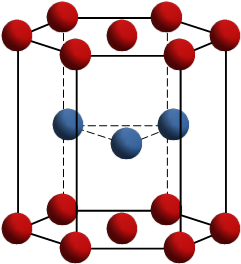
\includegraphics[width=0.3\textwidth]{./Bilder/hcp}
	\hspace{4ex}
	\subfloat{}
	\includegraphics[width=0.3\textwidth]{Bilder/krz}
	\caption{Kristallgitterstruktur der $\alpha$-Phase (hex) und $\beta$-Phase (krz)}
	\label{fig:Kristallgitter}
\end{figure}


\subsection{Klassifizierung von Titan und Titanlegierungen}

Da reines Titan wie alle anderen Metalle keine hohe Festigkeit besitzt, werden Legierungen hergestellt, um die mechanischen Eigenschaften gezielt zu verändern. Die in der Industrie erhältlichen Titanlegierungen werden daher in verschiedene Klassen eingeteilt. Den $\alpha$-, $\alpha+\beta$- sowie den $\beta$-Legierungen. Die $\alpha+\beta$-Legierungen werden zusätzlich in near-$\alpha$- und near-$\beta$-Legierungen aufgeteilt. Die Klassifikation hängt vom Typ und der Menge der Legierungselemente ab. Des weiteren gibt es technisch reines Titan (CP-Titanium), das zunächst nur im amerikanischen Normungssystem ASTM (American Standard for Testing of Materials) in vier Klassen, den sogenannten CP-Grades 1, 2, 3 und 4 eingeteilt wurde. Dieses Bezeichnungssystem wurde später übersetzt und in deutsche und europäische Normen übernommen.
Die für Titanwerkstoffe typischen Legierungselemente werden in vier Kategorien eingeteilt, die sich in ihrer Wirkungsweise unterscheiden. 
Als $\alpha$-Stabilisatoren werden Legierungselemente wie Aluminium (Al), Sauerstoff (O) und Stickstoff (N) bezeichnet, die zu einer Einschnürung des $\beta$-Phasengebietes führen und die $\beta$-Transus-Temperatur erhöhen.
Des weiteren gibt es die $\beta$-Stabilisatoren, die das $\beta$-Phasengebiet erweitern und die $\beta$-Transus-Temperatur verringern. Man unterscheidet bei den $\beta$-Stabilisatoren zwischen $\beta$-isomorphen und $\beta$-eutektoiden Stabilisatoren. Zu den $\beta$-isomorph wirkenden Stabilisatoren gehören die Elemte Molybdän (Mo), Vanadium (V), Niob (Nb) und Tantal (Ta). Diese erweitern das $\beta$-Phasengebiet bis zur Raumtemperatur. 
Zu den $\beta$-eutektoiden-Stabilisatoren gehören Elemente wie Eisen (Fe), Chrom (Cr), Kupfer (Cu), Mangan (Mn) und Silizium (Si). Bei diesen Stabilisatoren kommt es unterhalb einer elementabhängigen Grenztemperatur zu einer eutektoiden Reaktion, die zu einer Ausscheidung einer zusätzlichen Phase führt. Diese Verbindung liegt entweder elementar oder intermetallisch vor.
Die Elemente  Zinn (Sn) und Zirkon (Zr) werden häufig als neutral bezeichnet, da diese nur eine sehr geringe $\alpha$-stabilisierende Wirkung haben.

\begin{figure}[h]
	\centering
%	\includegraphics[width=1.0\linewidth]{/Bilder/Tabelle 1}
	\includegraphics[width=1.0\linewidth]{Bilder/Tabelle 1.png}
	\caption[Tabelle 1]{Tabelle typischer Legierungselemte und ihre stabilisierende Wirkung \cite{Boyer.2007,M.J.Donachie.2010}}
	\label{fig:tabelle-1}
\end{figure}


Bei einer Wärmebehandlung von near-$\alpha$-, $\alpha$+$\beta$- oder metastabilen $\beta$-Titanlegierungen im Zweiphasengebiet (also unterhalb der $\beta$-Transus Temperatur) kommt es bei ausreichend langen Glühzeiten zum sogenannten Element Partitioning \cite{Lutjering.2007}. Dabei diffundieren die $\alpha$-stabilisierenden Elemente in die $\alpha$-Phase und die $\beta$-stabilisierenden Elemente in die $\beta$-Phase, so dass die lokale chemische Zusammensetzung der jeweiligen Phasen von der globalen chemischen Zusammensetzung einer Legierung abweichen kann.

\begin{figure}[h]
	\centering
	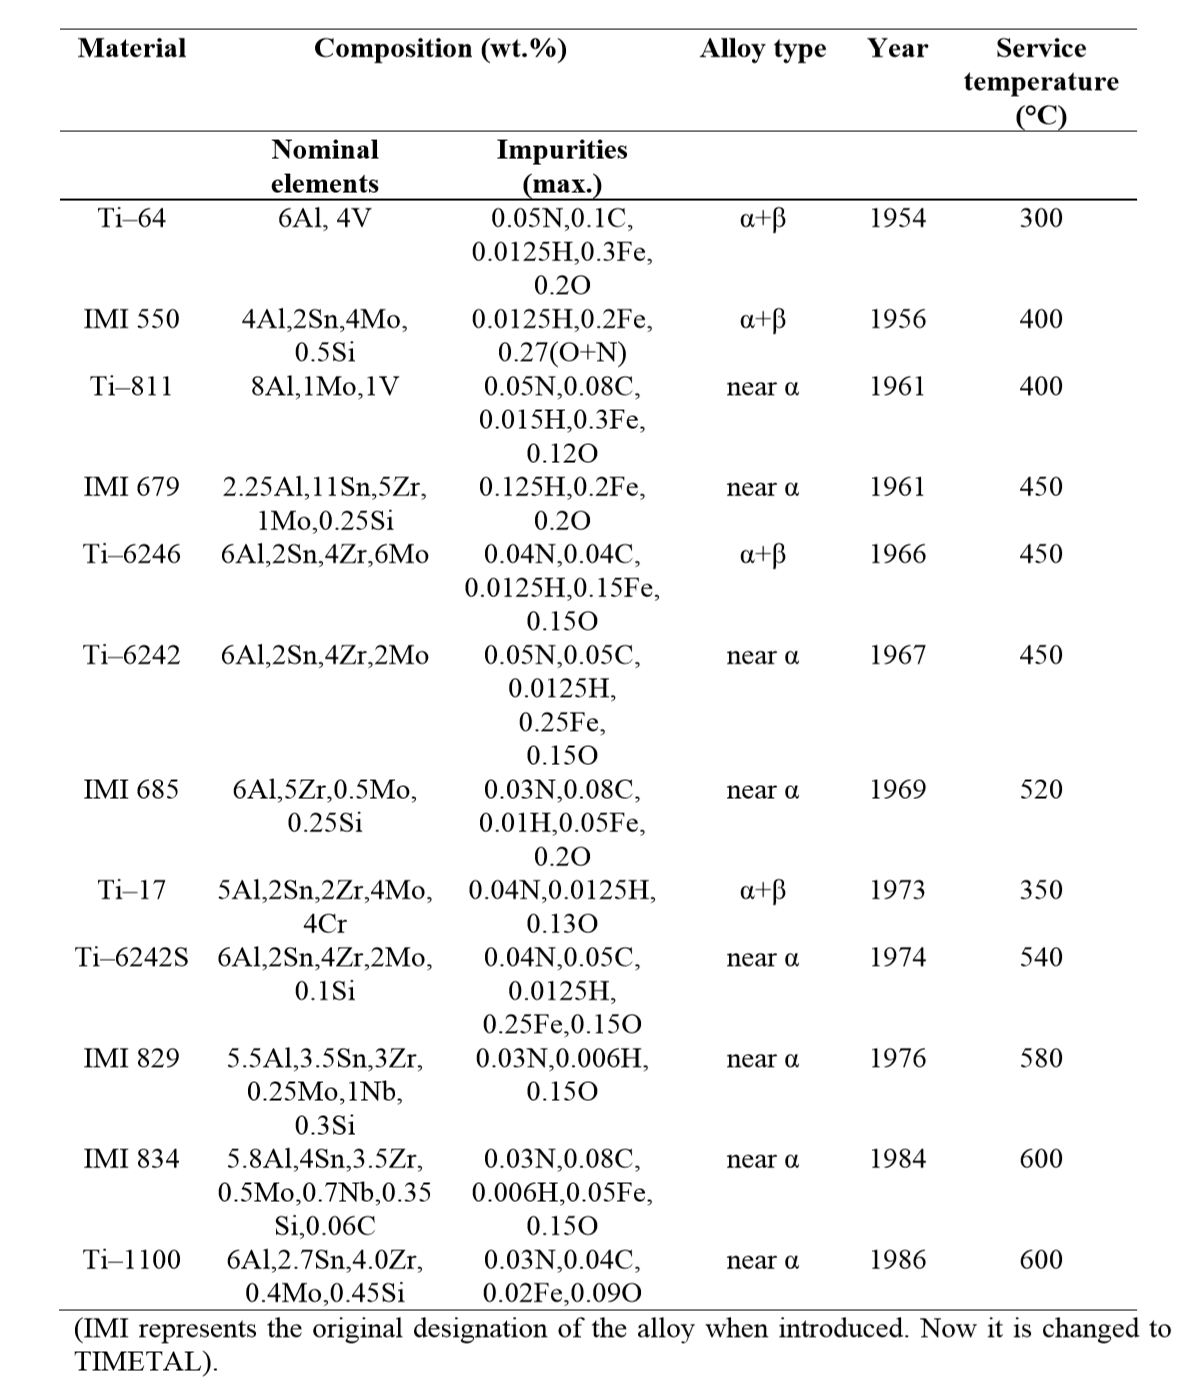
\includegraphics[width=0.8\linewidth]{./Bilder/Tabelle 2.png}
	\caption[Tabelle 2]{kommerziell genutzte Titanlegierungen nach ihren Erscheinungsjahren, der chemischen Zusammensetzung und maximalen Einsatztemperatur \cite{D.EylonS.FujishiroF.H.Froes.1984,P.A.Blenkinsop.1984,A.K.Gogia.2005}}
	\label{fig:tabelle-2}
\end{figure}

\paragraph{CP-Titanium} 
Zu reinem Titan (\textit{commercially pure}, CP) werden keine Legierungselemente dazugegeben, jedoch sind Begleitelemente wie Sauerstoff und Eisen in bestimmten Mengen nicht zu vermeiden. In welche Klasse technisch reines Titan eingeordnet wird, hängt von der Konzentration der Begleitelemente ab. Es gibt 4 Klassen, die sogenannten CP-Grades \cite{C.Leyens.2005}.

\paragraph{$\alpha$- und near-$\alpha$-Legierungen}
Wenn $\alpha$-Stabilisatoren dem reinen Titan hinzulegiert werden, führt dies zu einer stabilen $\alpha$-Phase bei Raumtemperatur. Daher werden sie als $\alpha$-Legierungen bezeichnet. Wird ein kleiner Anteil an $\beta$-Stabilisatoren ( 1--2 Gew.\%) hinzugefügt, führt dies zu einer near-$\alpha$-Legierung mit einem kleinen Anteil an $\beta$-Phase (\textless5\%) bei Raumtemperatur. Ein typisches Beispiel einer $\alpha$-Legierung ist Ti–5Al–2.5Sn. Zu den Vertretern von near-$\alpha$-Legierungen gehören Ti–8Al–1Mo–1V und Ti–6Al–2Sn–4Zr–2Mo. Der Aluminiumgehalt in diesen Legierungen wird typischerweise unter 9 \% gehalten, da es sonst zu $Ti_{3}Al$-Ausscheidungen und dadurch zu Versprödungen kommen kann \cite{C.Leyens.2005,Lutjering.2007,Boyer.2007,M.J.Donachie.2010}.

\paragraph{$\alpha$+$\beta$-Legierungen}
Diese Legierungen bilden die erste Untergruppe der zweiphasigen Titanlegierungen. Bei Raumtemperatur besitzen sie zwischen 5\% und 95\% $\beta$-Phase im Gefüge. Sie können dabei vollständig oder teilweise martensitsch ($\alpha'$- oder $\alpha''$-Phase) umwandeln. Die bekanntesten $\alpha$+$\beta$ Legierungen sind Ti–6Al–4V und Ti–6Al–2Sn–4Zr–6Mo \cite{C.Leyens.2005,Lutjering.2007,Boyer.2007,M.J.Donachie.2010}.

\paragraph{Metastabile $\beta$-Legierungen}
Die zweite Untergruppe der zweiphasigen Titanlegierungen bilden die metastabilen $\beta$-Legierungen. Wie die $\alpha$+$\beta$-Legierungen besitzen sie zwischen 5\% und 95\% $\beta$-Phase im Gefüge, zeigen dagegen keine martensitische Umwandlung. Sie sind jedoch ausscheidungshärtbar und enthalten größere Gehalte an $\beta$-stabilisieren Elementen, so dass die Martensitstarttemperatur unterhalb Raumtemperatur liegt \cite{C.Leyens.2005,Lutjering.2007,Boyer.2007,M.J.Donachie.2010}. 

\paragraph{Near-$\beta$- und $\beta$-Legierungen}
Diese Legierungen enthalten ca. 10--15 \% $\beta$-Stabilisatoren neben einem kleinen Anteil an $\alpha$-Stabilisatoren. Sie haben dadurch einen größeren Anteil an $\beta$-phase bei Raumtemperatur und werden deshalb near-$\beta$-Legierungen genannt. Im Gegensatz dazu, haben die $\beta$-Legierungen einen sehr hohen Volumenanteil an $\beta$-Phase. Ein Beispiel für near-$\beta$-Legierungen ist Ti–5Al–2Sn–2Zr–4Cr–4Mo. Zu den Vertretern der $\beta$-Legierungen gehört Ti–15Mo–2.7Nb–3Al–0.2Si \cite{Boyer.2007,M.J.Donachie.2010}.

\subsection{Herstellung von Titanlegierungen}
Titan kommt in der Natur nicht als reines Metall vor, sondern wird aus Titanerzen gewonnen. Die wirtschaftlich bedeutenden Erze sind Rutil ($TiO_2$) und Ilmenit ($FeTiO_3$), welche in allen Erdteilen zu finden sind. Einen Überblick über den Herstellungsprozess vom Erz bis zum Endprodukt ist in Abbildung \ref{fig:abbildung-2} gegeben. Momentan ist das einzige Verfahren, um wirtschaftlich bedeutsame Mengen an Titan herstellen zu können, der Kroll-Prozess (bzw. der Hunter-Prozess) \cite{C.Leyens.2005}. Beim Kroll-Prozess wird zunächst in einem Verhüttungsprozess das Titanerz von den Eisenoxiden getrennt. Dabei entsteht Roheisen, dass zur Produktion von hochwertigen Stählen genutzt wird, 
sowie Schlacke mit einem Titanoxidgehalt von etwa 80 -- 90 \%, die für die weitere Titangewinnung verwendet wird. Das in der Schlacke vorhandene Titanoxid wird unter der Verwendung von Chlorgas in mehreren Prozessschritten zu Titantetrachlorid ($TiCl_4$) umgesetzt. Dabei findet teilweise eine Rückreaktion zu $TiO_2$ statt, da Titan eine hohe Affinität zu Sauerstoff besitzt. Das Titantetrachlorid wird anschließend mit Magnesium zum sogenannten Titanschwamm (Sponge) reduziert. Dieser wird dann durch Vakuumdestillation von Rückständen ($Mg$ und $MgCl_2$) befreit, aus dem Reaktionsgefäß gedrückt und zerkleinert. Der Titanschwamm wird dann unter Zusatz von Legierungselementen zu Elektroden verpresst, die in einem Vakuum-Lichtbogen-Umschmelzprozess (Vacuum-Arc-Remelting, kurz VAR), zu einem Block, dem Ingot, umgeschmolzen werden. Diese Ingots können dann weiterverarbeitet werden und zum Beispiel durch Techniken wie Schmieden oder Rollen zu Platten, Blechen und Streifen umgeformt werden.  

\begin{figure}[h]
	\centering
	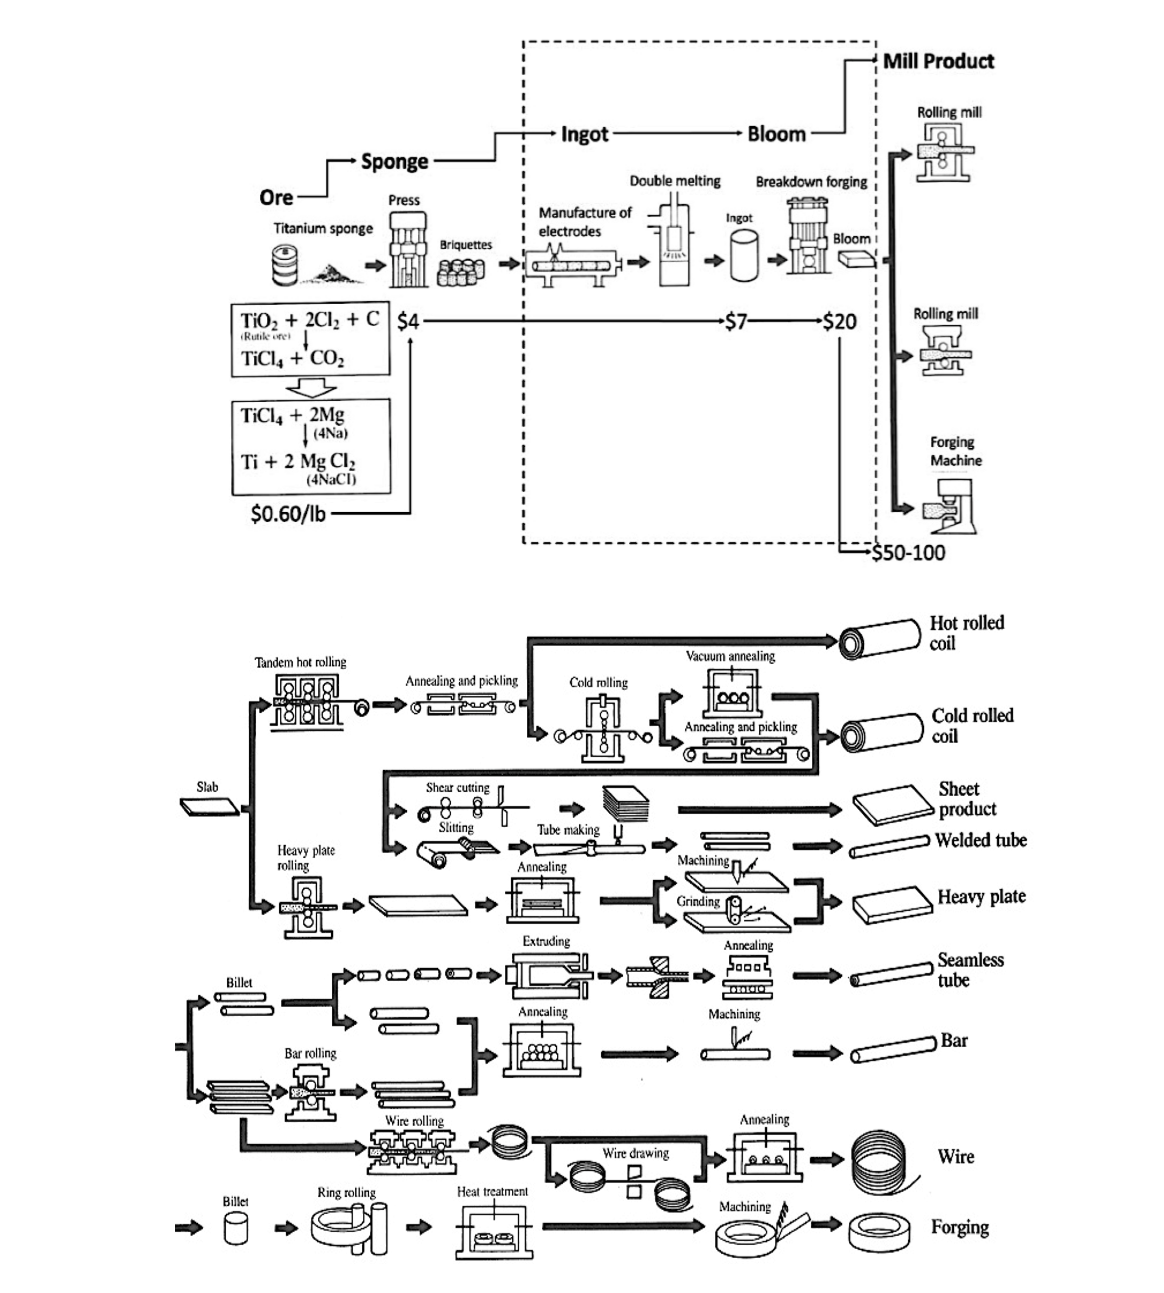
\includegraphics[width=0.7\linewidth]{./Bilder/Abbildung 2.png}
	\caption[Abbildung 2]{Überblick der Produktionsroute vom Erz zum Endprodukt \cite{M.J.Donachie.2010}}
	\label{fig:abbildung-2}
\end{figure}

\pagebreak

\subsection{Mikrostrukturen in Titanlegierungen}
Im Bereich der Titanlegierungen gibt es vier Basis-Mikrostrukturen die geformt werden können. Es gibt Widmanstätten-, Bi-Modal/Duplex-, globulare und martensitische Gefüge. Die $\beta$-Transus Temperatur spielt dabei eine entscheidend, welche Gefüge sich bei den Legierungen einstellen. Zusätzlich spielt die Abkühlrate beim Gießen der Legierung, der Grad beim Heiß-/Kaltumformen, die Glühtemperatur und Haltezeit eine wichtige Rolle \cite{C.Leyens.2005,Lutjering.2007,Boyer.2007,M.J.Donachie.2010}.

Die Abbildung \ref{fig:abbildung-6} zeigt schematisch die Entstehung der Mikrostruktur von reinem Titan während des Gießprozesses. Es ist zu sehen, dass sich bei Abkühlung an der Luft unterhalb der Schmelztemperatur (1668$^\circ$C), $\beta$-Phase in Form von Dendriten ausscheidet und zu kompletten $\beta$-Körnern heranwächst. Bei weiterer Abkühlung bis unter $\beta$-Transus (882$^\circ$C für reines Titan), transformiert sich $\beta$ zu $\alpha$. Die $\alpha$-Phase wächst an den Korngrenzen und in Form von Lamellen ($\alpha$-Lamellen) in das vorherige $\beta$-Korn hinein. Wenn mehrere dieser $\alpha$-Lamellen in dieselbe Richtung wachsen, formen sich sogenannte $\alpha$-Kolonien. Diese Kolonien sind zufällig im vorherigen $\beta$-Korn verteilt und resultieren im sogenannten Widmannstättengefüge. Die Größe dieser mikrostrukturellen Formation ist abhängig von der Abkühlrate. Schnelles Abkühlen von unterhalb der $\beta$-Transus-Temperatur resultiert in feinen $\alpha$-Lamellen und kleinen $\alpha$-Kolonien. Langsames Abkühlen führt zu breiteren Lamellen und gröberen Kolonien \cite{C.Leyens.2005,Lutjering.2007,Boyer.2007,M.J.Donachie.2010}. 

\pagebreak

\begin{figure}[h]
	\centering
	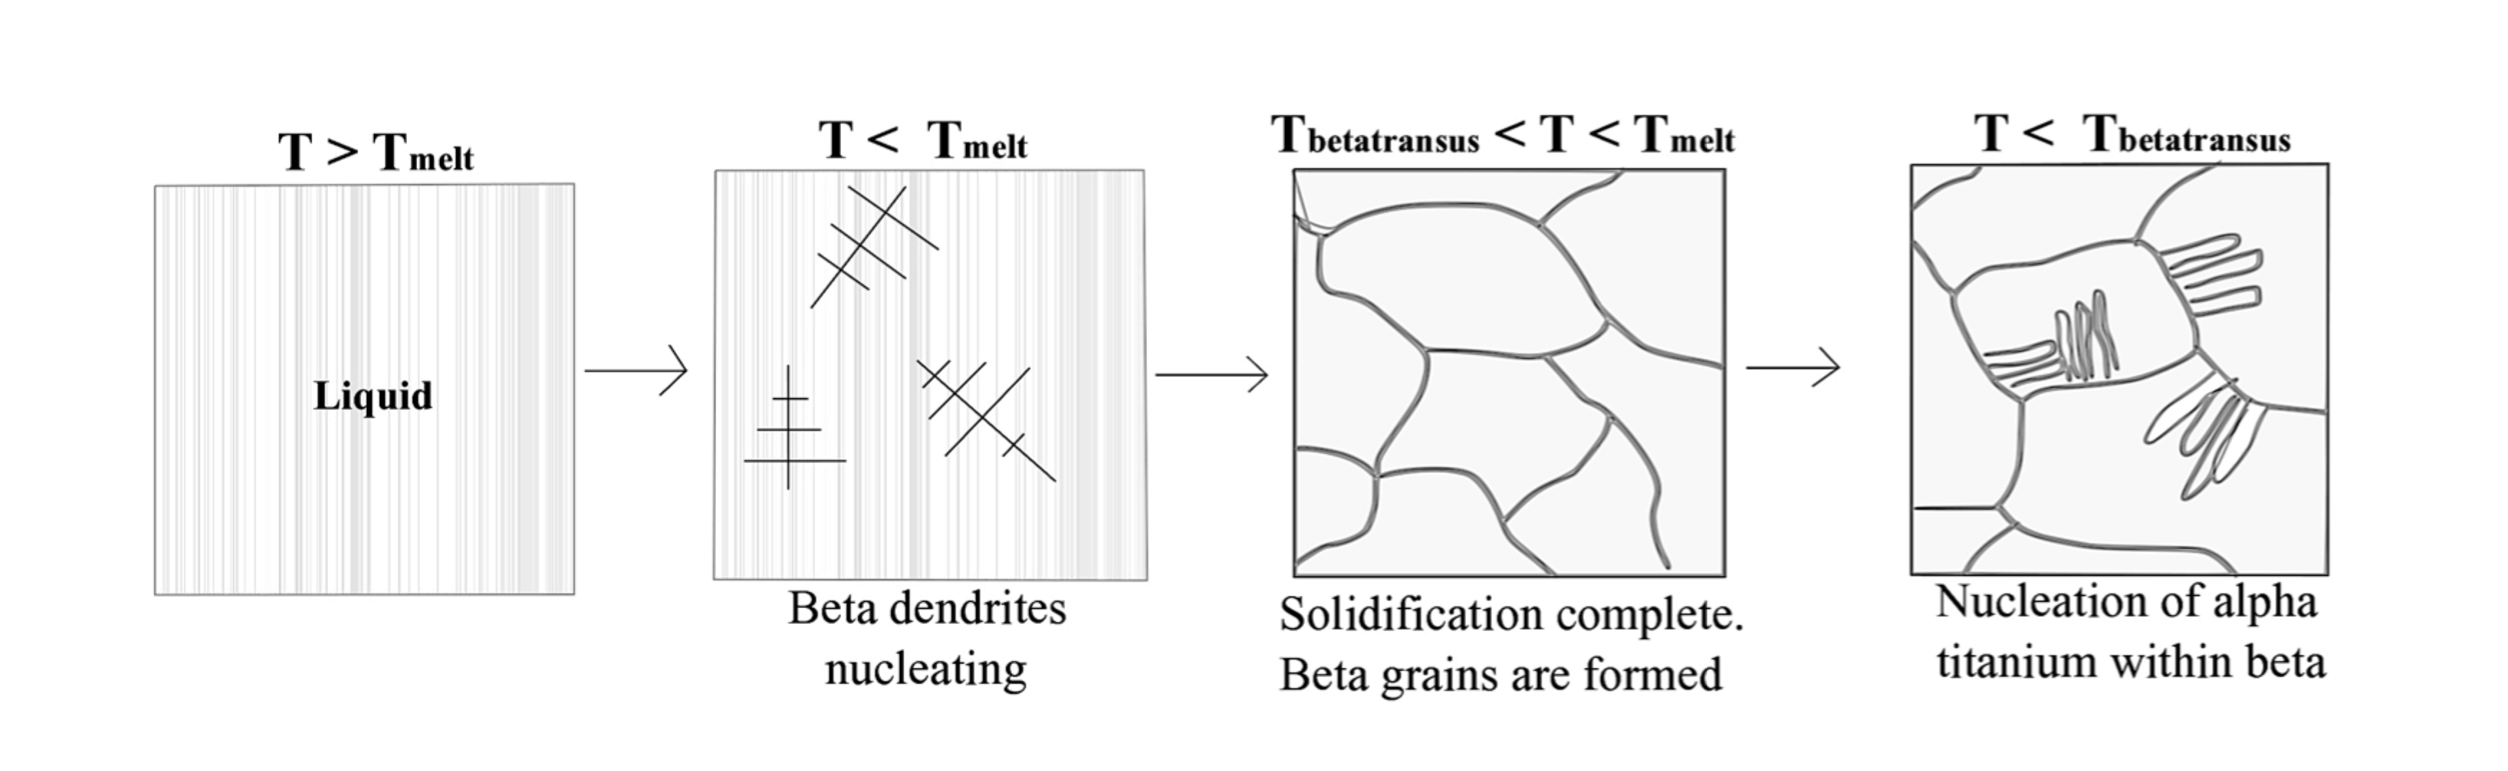
\includegraphics[width=0.8\linewidth]{./Bilder/Abbildung 6.png}
	\caption[Abbildung 6]{schematische Darstellung der Entstehung der Mikrostruktur in reinem Titan, abgekühlt aus dem flüssigem Zustand bis unter Beta-Transus \cite{M.J.Berminghametal..2007}}
	\label{fig:abbildung-6}
\end{figure}


Mikrostrukturen, die man während des Gießens erhält, sind sehr grob und besitzen eine geringe Festigkeit. Daher werden diese Mikrostrukturen mithilfe von thermo-mechanischen Prozessschritten modifiziert. Dazu gehören die Verfeinerung der Mikrostruktur durch Rekristallisation oder die Formation neuer Mikrostrukturen durch Kornwachstum \cite{C.Leyens.2005,Lutjering.2007,Boyer.2007,M.J.Donachie.2010}.
Typische thermo-mechanische Prozessschritte für Near-$\alpha$- und $\alpha+\beta$-Legierungen beinhalten die Homogenisierung (solution heat treatment), Deformation, Rekristallisation, das Altern (ageing) und Spannungsarmglühen (stress relief annealing) \cite{C.Leyens.2005,Lutjering.2007,Boyer.2007}. Ein Beispiel für den Ablauf dieser Prozessschritte ist in Abbildung \ref{fig:abbildung-7} dargestellt. Man unterscheidet dabei zwischen lamellaren, bimodalen und globularen Mikrostrukturen. 

\begin{figure}[h]
	\centering
	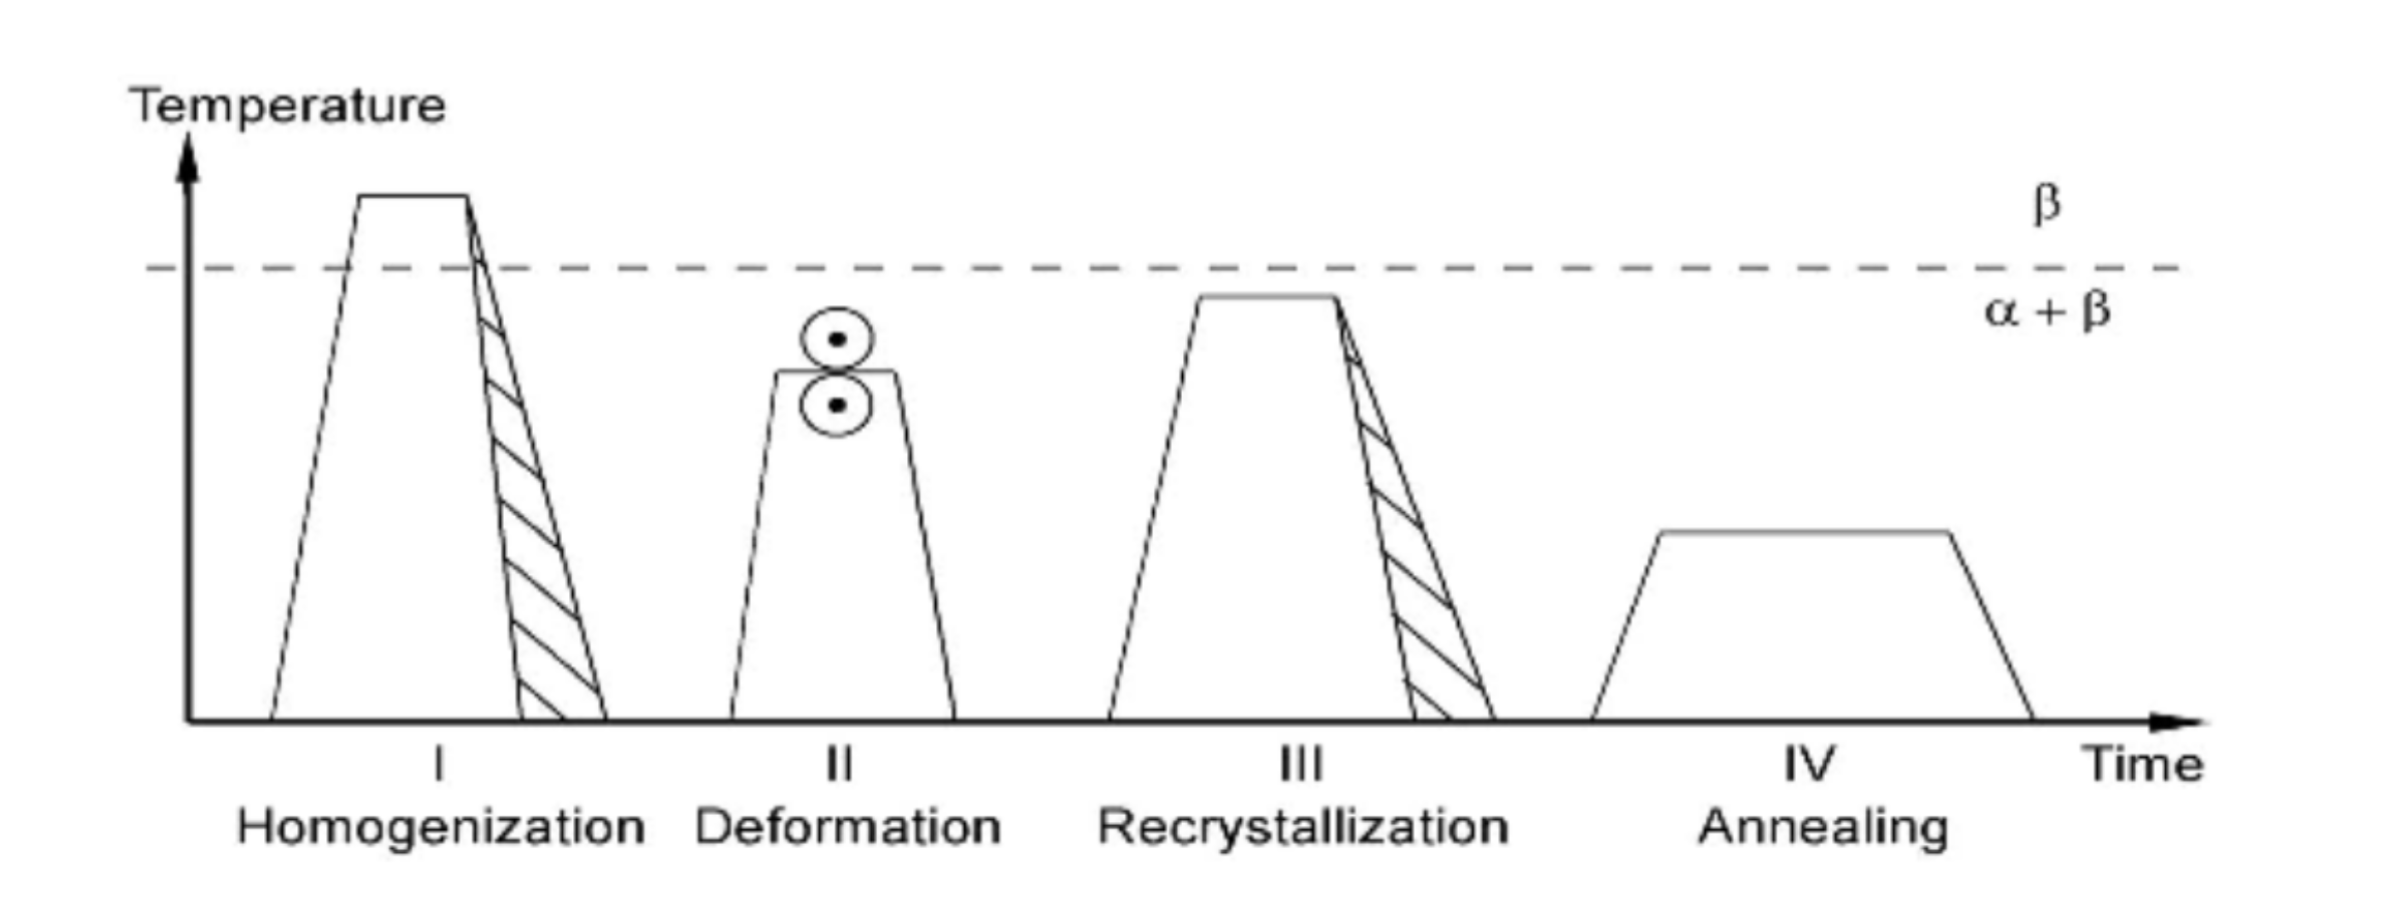
\includegraphics[width=0.9\linewidth]{./Bilder/Abbildung 7.png}
	\caption[Abbildung 7]{Prozessschritte für bimodale Mikrostrukturen von $\alpha$+$\beta$-Legierungen schematisch \cite{M.PetersJ.KumpfertC.WardC.Leyens.2003}}
	\label{fig:abbildung-7}
\end{figure}

Eine kurze Beschreibung dieser Mikrostrukturen ist im folgenden aufgeführt.

\begin{itemize} 
	\item lamellare Mikrostruktur: entsteht bei einer Wärmebehandlung mit etwa $30-50 ^\circ C$ über der $\beta$-Transus-Temperatur, nach plastischer Deformation im $\beta$- und $\alpha$+$\beta$-Phasengebiet, um große $\beta$-Körner zu vermeiden. Die resultierende Mikrostruktur ist abhängig von der Abkühlrate nach dem Glühen. So resultiert aus einer geringen Abkühlrate eine grobe Widmannstätten-Mikrostruktur, mit breiten $\alpha$-Lamellen, dickeren Korngrenzen und größeren $\alpha$-Kolonien. 

\begin{figure}[h]
	\centering
	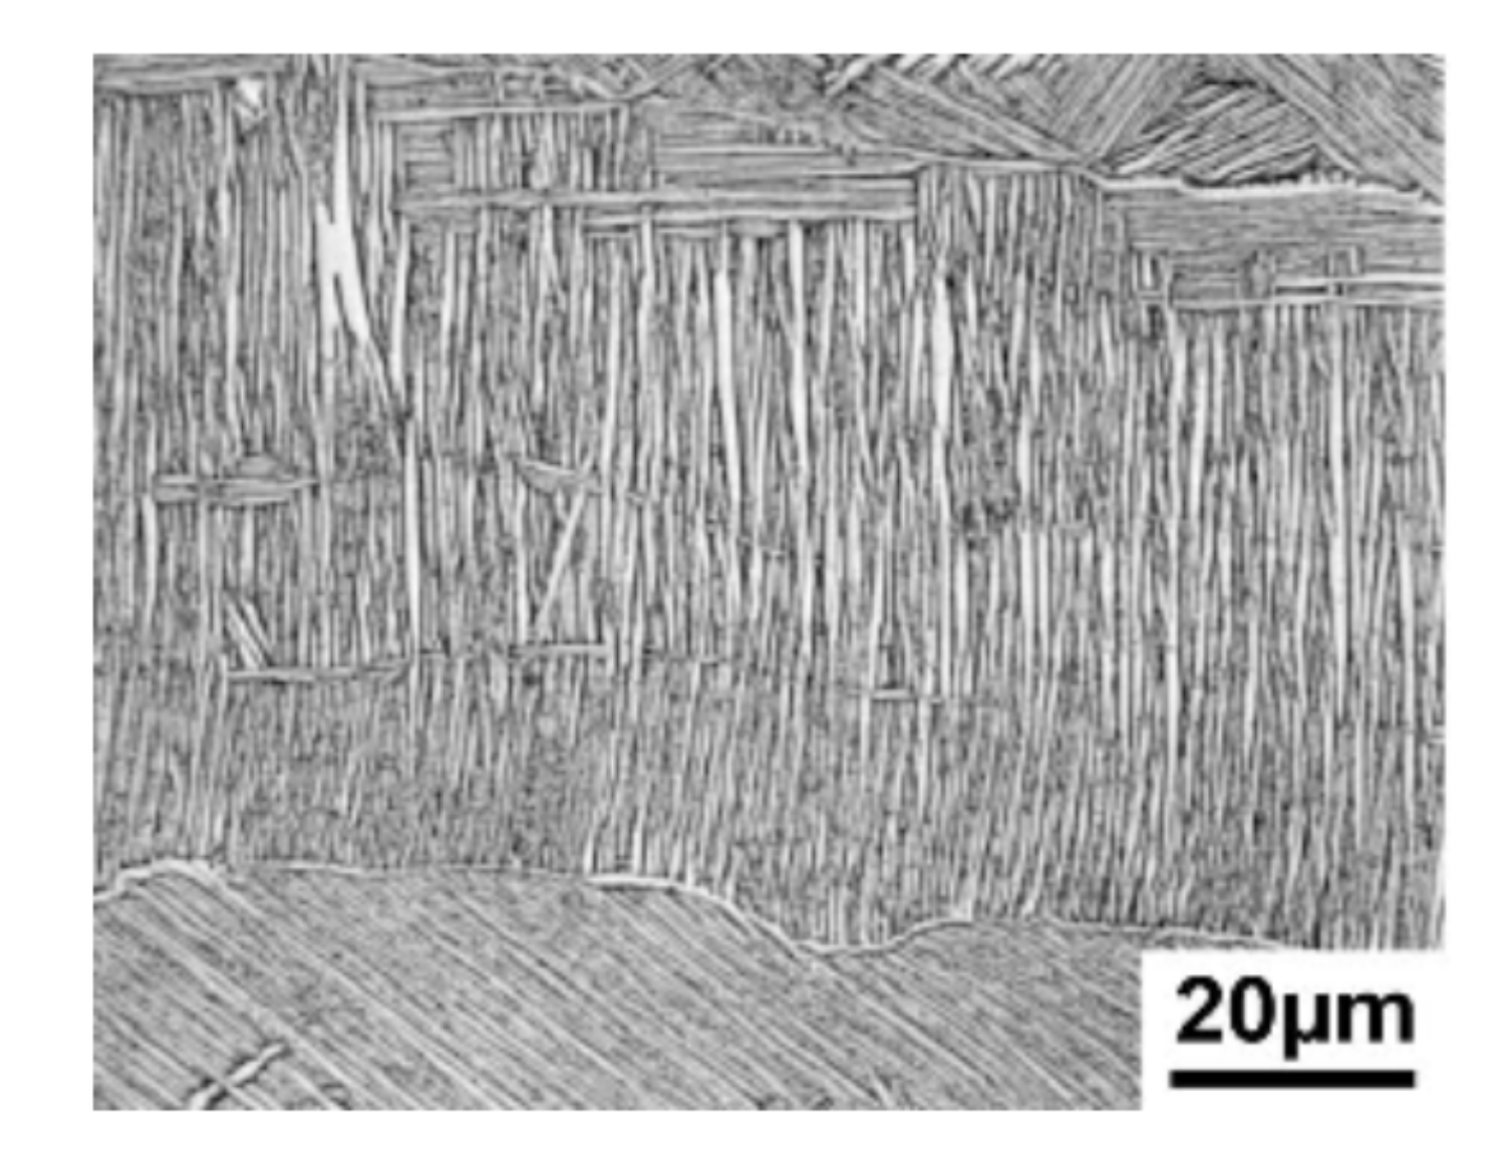
\includegraphics[width=0.7\linewidth]{./Bilder/Abbildung 3.png}
	\caption[Abbildung 3]{lamellare Mikrostruktur von Ti-6242, Abkühlrate ca 100$^\circ$C/min, LM \cite{Lutjering.2007}}
	\label{fig:abbildung-3}
\end{figure}

\pagebreak

\item bimodale Mikrostruktur: entsteht nach umfangreicher Deformation im $\alpha+\beta$-Phasengebiet und einer Wärmebehandlung unterhalb der $\beta$-Transus-Temperatur. Dies resultiert in globularem Primär-$\alpha$ ($\alpha_p$), transformierten $\beta$ und $\alpha$ entlang der Korngrenzen der vorherigen $\beta$-Körner. Das transformierte $\beta$ besteht aus einer Widmannstättenstruktur, mit feinen $\alpha$-Lamellen, die in $\alpha$-Kolonien angeordnet sind. Die Größe dieser mikrostrukturellen Bestandteile hängen von der Glühtemperatur, Abkühlrate, sowie der Temperatur und Zeit bei der Deformation ab. Der Volumenanteil von primären $\alpha$ hängt hauptsächlich von der Temperatur beim Glühen und der Temperatur bei der Deformation ab \cite{Lutjering.2007}.

\begin{figure}[h]
	\centering
	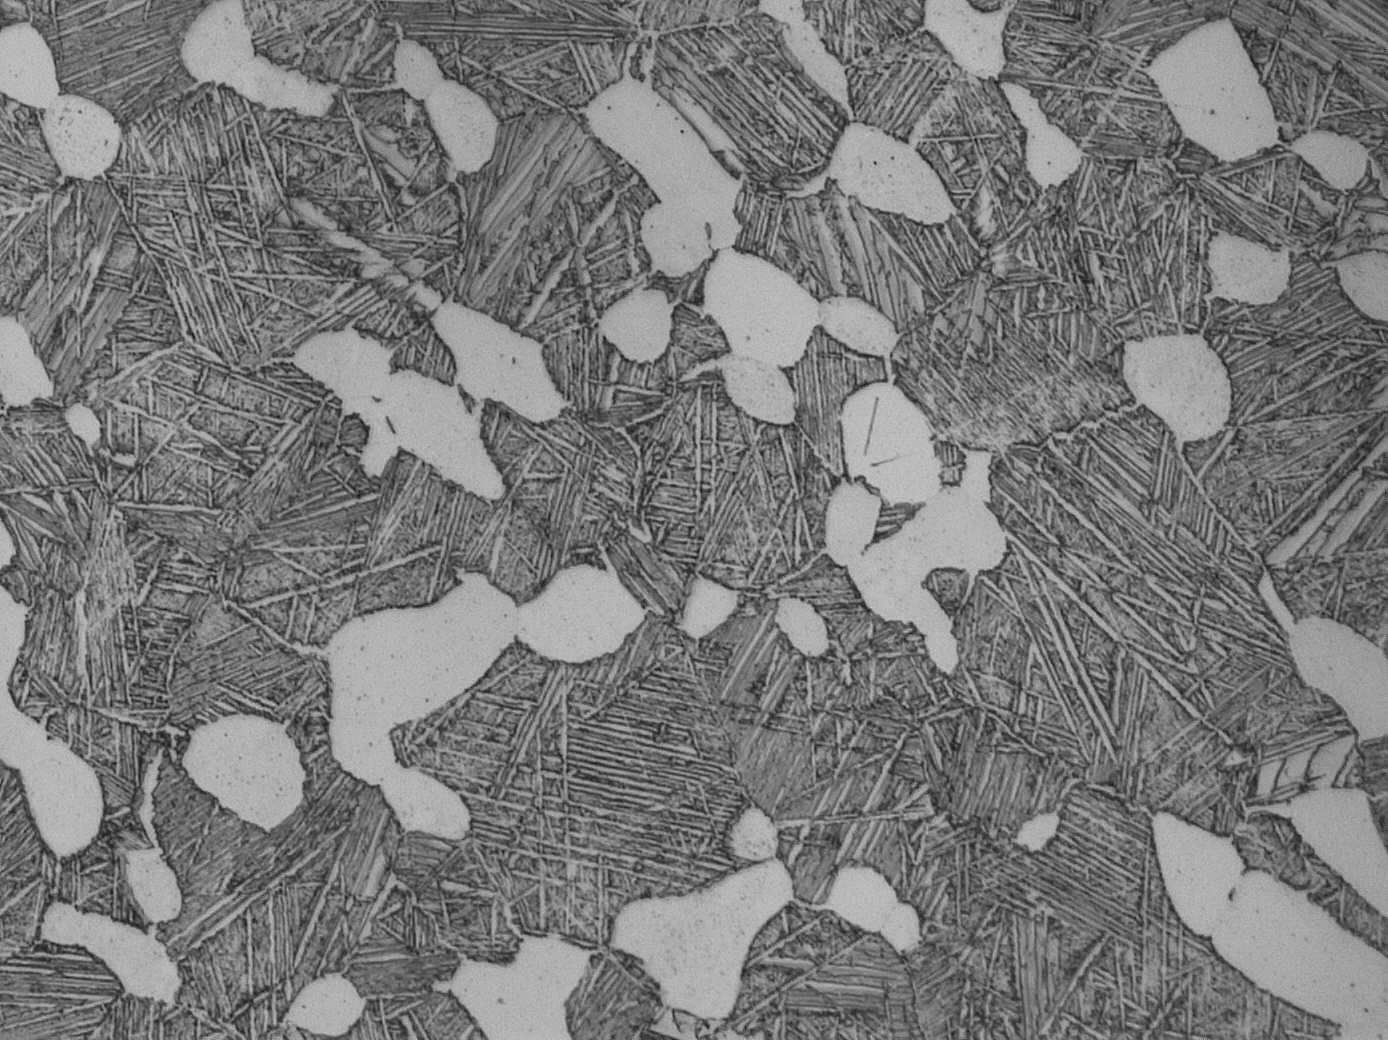
\includegraphics[width=0.7\linewidth]{./Bilder/Abbildung 4.jpg}
	\caption[Abbildung 4]{bimodale Mikrostruktur Ti-6242, \SI{20}{\micro\metre}}
	\label{fig:abbildung-4}
\end{figure}


\item globulare Mikrostruktur: wird erreicht durch eine mechanische Bearbeitung und Lösungsglühen im Zweiphasengebiet. Durch den Rekristallisationsprozesses zerbricht das lamellare $\alpha$ in globulares. Verlängertes Glühen vergröbert die globulare Mikrostruktur \cite{Lutjering.2007}. 
\end{itemize} 

\begin{figure}[h]
	\centering
	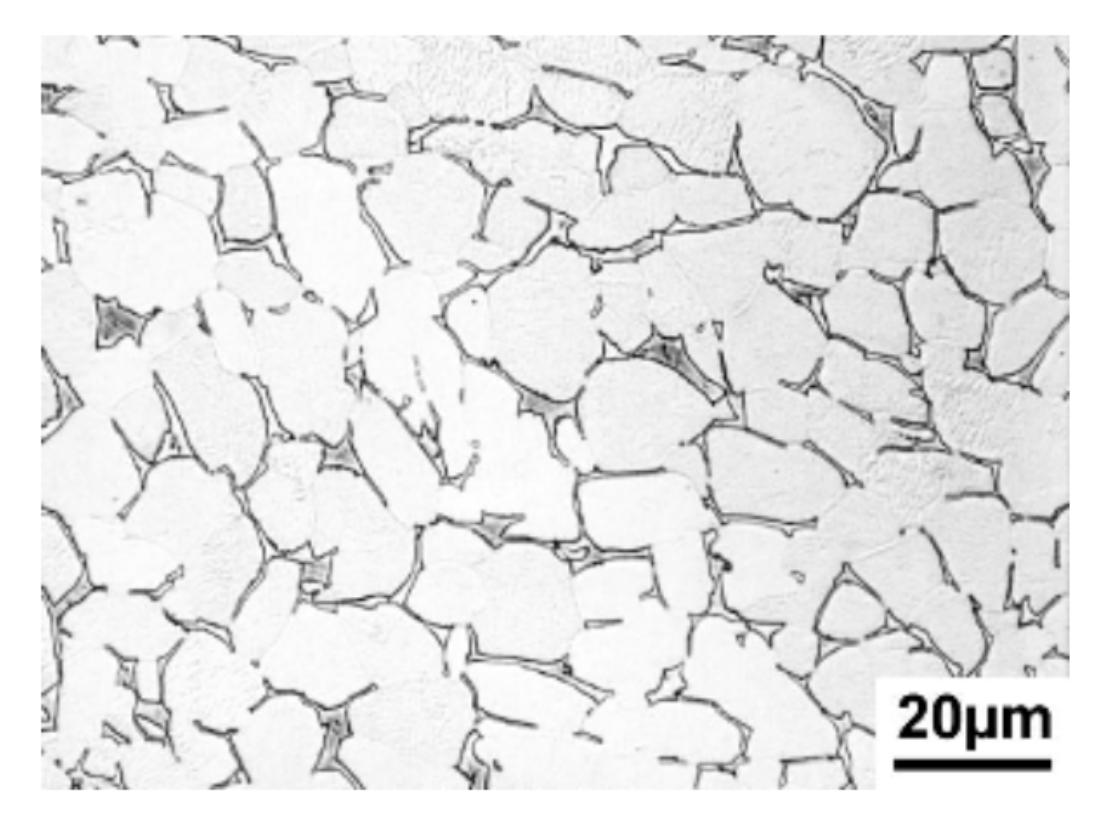
\includegraphics[width=0.7\linewidth]{./Bilder/Abbildung 5.png}
	\caption[Abbildung 5]{globulare Mikrostruktur von Ti-6242, LM \cite{Lutjering.2007}}
	\label{fig:abbildung-5}
\end{figure}



\subsection{Mechanische Eigenschaften von Titanlegierungen}

Dieser Abschnitt gibt einen Überblick über die typischen mechanischen Eigenschaften der verschiedenen Klassen von Titanlegierungen. Des Weiteren werden die Einflüsse von verschiedenen Mikrostrukturen auf diese Eigenschaften aufgezeigt.

\paragraph{$\alpha$-Legierungen}  
CP-Titanium ist das am weitesten genutzte unter den $\alpha$-Legierungen. Sie besitzen eine annehmbare Zugfestigkeit und gute Duktilität bei Raumtemperatur. Des Weiteren besitzen sie eine geringe Dichte, eine gute Härte, sehr gute Kriechbeständigkeit und Schweißbarkeit. Die Besonderheit dieser Legierungen ist, dass sie bei kryogenen Temperaturen keine Versprödung zeigt \cite{C.Leyens.2005,Lutjering.2007,M.J.Donachie.2010}. 

\paragraph{Near-$\alpha$-Legierungen} 
zeichnen sich durch eine hohe Kriech- und Oxidationsbeständigkeit aus. Ti-6242 ist die am häufigsten kommerziell eingesetzte Legierung für Temperaturen bis zu $450 ^\circ C$. 
Sie wurde als Ergänzung zu der bekannten Ti-64 Legierung entwickelt und erhöhte dadurch das Temperaturlimit. In den meisten Near-$\alpha$-Legierungen befindet sich Silikon (siehe Tabelle \ref{fig:tabelle-2}) als Legierungselement, um die Temperaturbeständigkeit zu verbessern \cite{C.Leyens.2005,Lutjering.2007}. 

\paragraph{$\alpha+\beta$-Legierungen} besitzen eine höhere Festigkeit, Härte und Korrosionsbeständigkeit. Dagegen ist die Duktilität und die Kriechbeständigkeit bei hohen Temperaturen schlechter als bei near-$\alpha$-Legierungen. Diese Legierungen haben eine hohe Festigkeit bei Raumtemperatur, sowie gute Heißumformeigenschaften. Typischerweise besitzen diese Legierungen 10 -- 15 \% $\beta$-Phase bei Raumtemperatur. Bei über 20 \% werden sie schwer schweißbar. Ti-64 ist die meistverwendete $\alpha+\beta$-Legierung und besitzt eine gute Kombination aus Festigkeit und Ermüdungseigenschaften bis zu $300 ^\circ C$ \cite{Boyer.2007,M.J.Donachie.2010}. 

\paragraph{Near-$\beta$- and $\beta$-Legierungen} besitzen eine sehr gute Härtbarkeit und Formbarkeit über ein weites Band an Temperaturen. Sie haben eine hohe Festigkeit und Härte. 
$\beta$-Legierungen zeigen eine erhöhte Härte, Bruchzähigkeit und Korrosionsbeständigkeit. 
Im Gegensatz zu den anderen Legierungen, haben sie eine höhere Dichte und eine geringere Duktilität. $\beta$-Legierungen sind sehr anfällig für Kaltversprödung und daher nicht geeignet für den Einsatz bei niedrigen Temperaturen \cite{C.Leyens.2005,Lutjering.2007,M.J.Donachie.2010}. 

Die beschriebenen Eigenschaften der verschiedenen Legierungen sind jedoch abhängig von den zugefügten Legierungselementen sowie dem gewählten Herstellungsprozess.
Die Legierungselemente entscheiden größtenteils über die mechanischen und chemischen Eigenschaften (Korrosion, Oxidation) \cite{C.Leyens.2005,Lutjering.2007,M.J.Donachie.2010}.

Der Herstellungsprozess hat ebenfalls einen erheblichen Einfluss auf die mechanischen Eigenschaften der Legierungen. Durch verschiedene Wärmebehandlungen können dadurch unterschiedliche Mikrostrukturen eingestellt und ihre mikrostrukturellen Eigenschaften verändert werden \cite{C.Leyens.2005,Lutjering.2007,Boyer.2007,M.J.Donachie.2010}.

Wie im vorherigen Kapitel erwähnt, werden die Mikrostrukturen eingeteilt in lamellar, globular und bi-modal. Diese bestehen hauptsächlich aus $\alpha$- und $\beta$-Phase, welche in verschiedenen physischen Formen auftreten. Die wichtigsten Eigenschaften der Mikrostrukturen werden durch die Faktoren Primär $\alpha$, $\alpha$-Kolonien, der Korngrenzen sowie dem transformierten $\beta$ beeinflusst \cite{C.Leyens.2005,Lutjering.2007,Boyer.2007}. Der Effekt der Mikrostrukturen auf die mechanischen Eigenschaften, abhängig von der mikrostrukterellen Größe der Faktoren, ist in Tabelle \ref{fig:tabelle-3} aufgeführt. Die Größe der $\alpha$-Kolonien, welche aufgrund verschiedener Abkühlraten entstehen, ist der wichtigste mikrostrukturelle Faktor. Es hat sich gezeigt, dass eine Verringerung der Koloniegröße, zu einer Verringerung der effektiven Gleitebene führt. Dadurch wird die Streckgrenze erhöht und die Rissanfälligkeit verringert. Größere $\alpha$ Kolonien erhöhen dagegen den Widerstand gegen Ermüdungsrissausbreitung und die Bruchzähigkeit \cite{C.Leyens.2005,Lutjering.2007,M.J.Donachie.2010}. Die Größe der $\alpha$-Kolonien wird durch die Größe des ursprünglichen $\beta$-Korns limitiert. Daher führen größere $\beta$-Körner auch zu einer besseren Kriechbeständigkeit.

\begin{figure}[h]
	\centering
	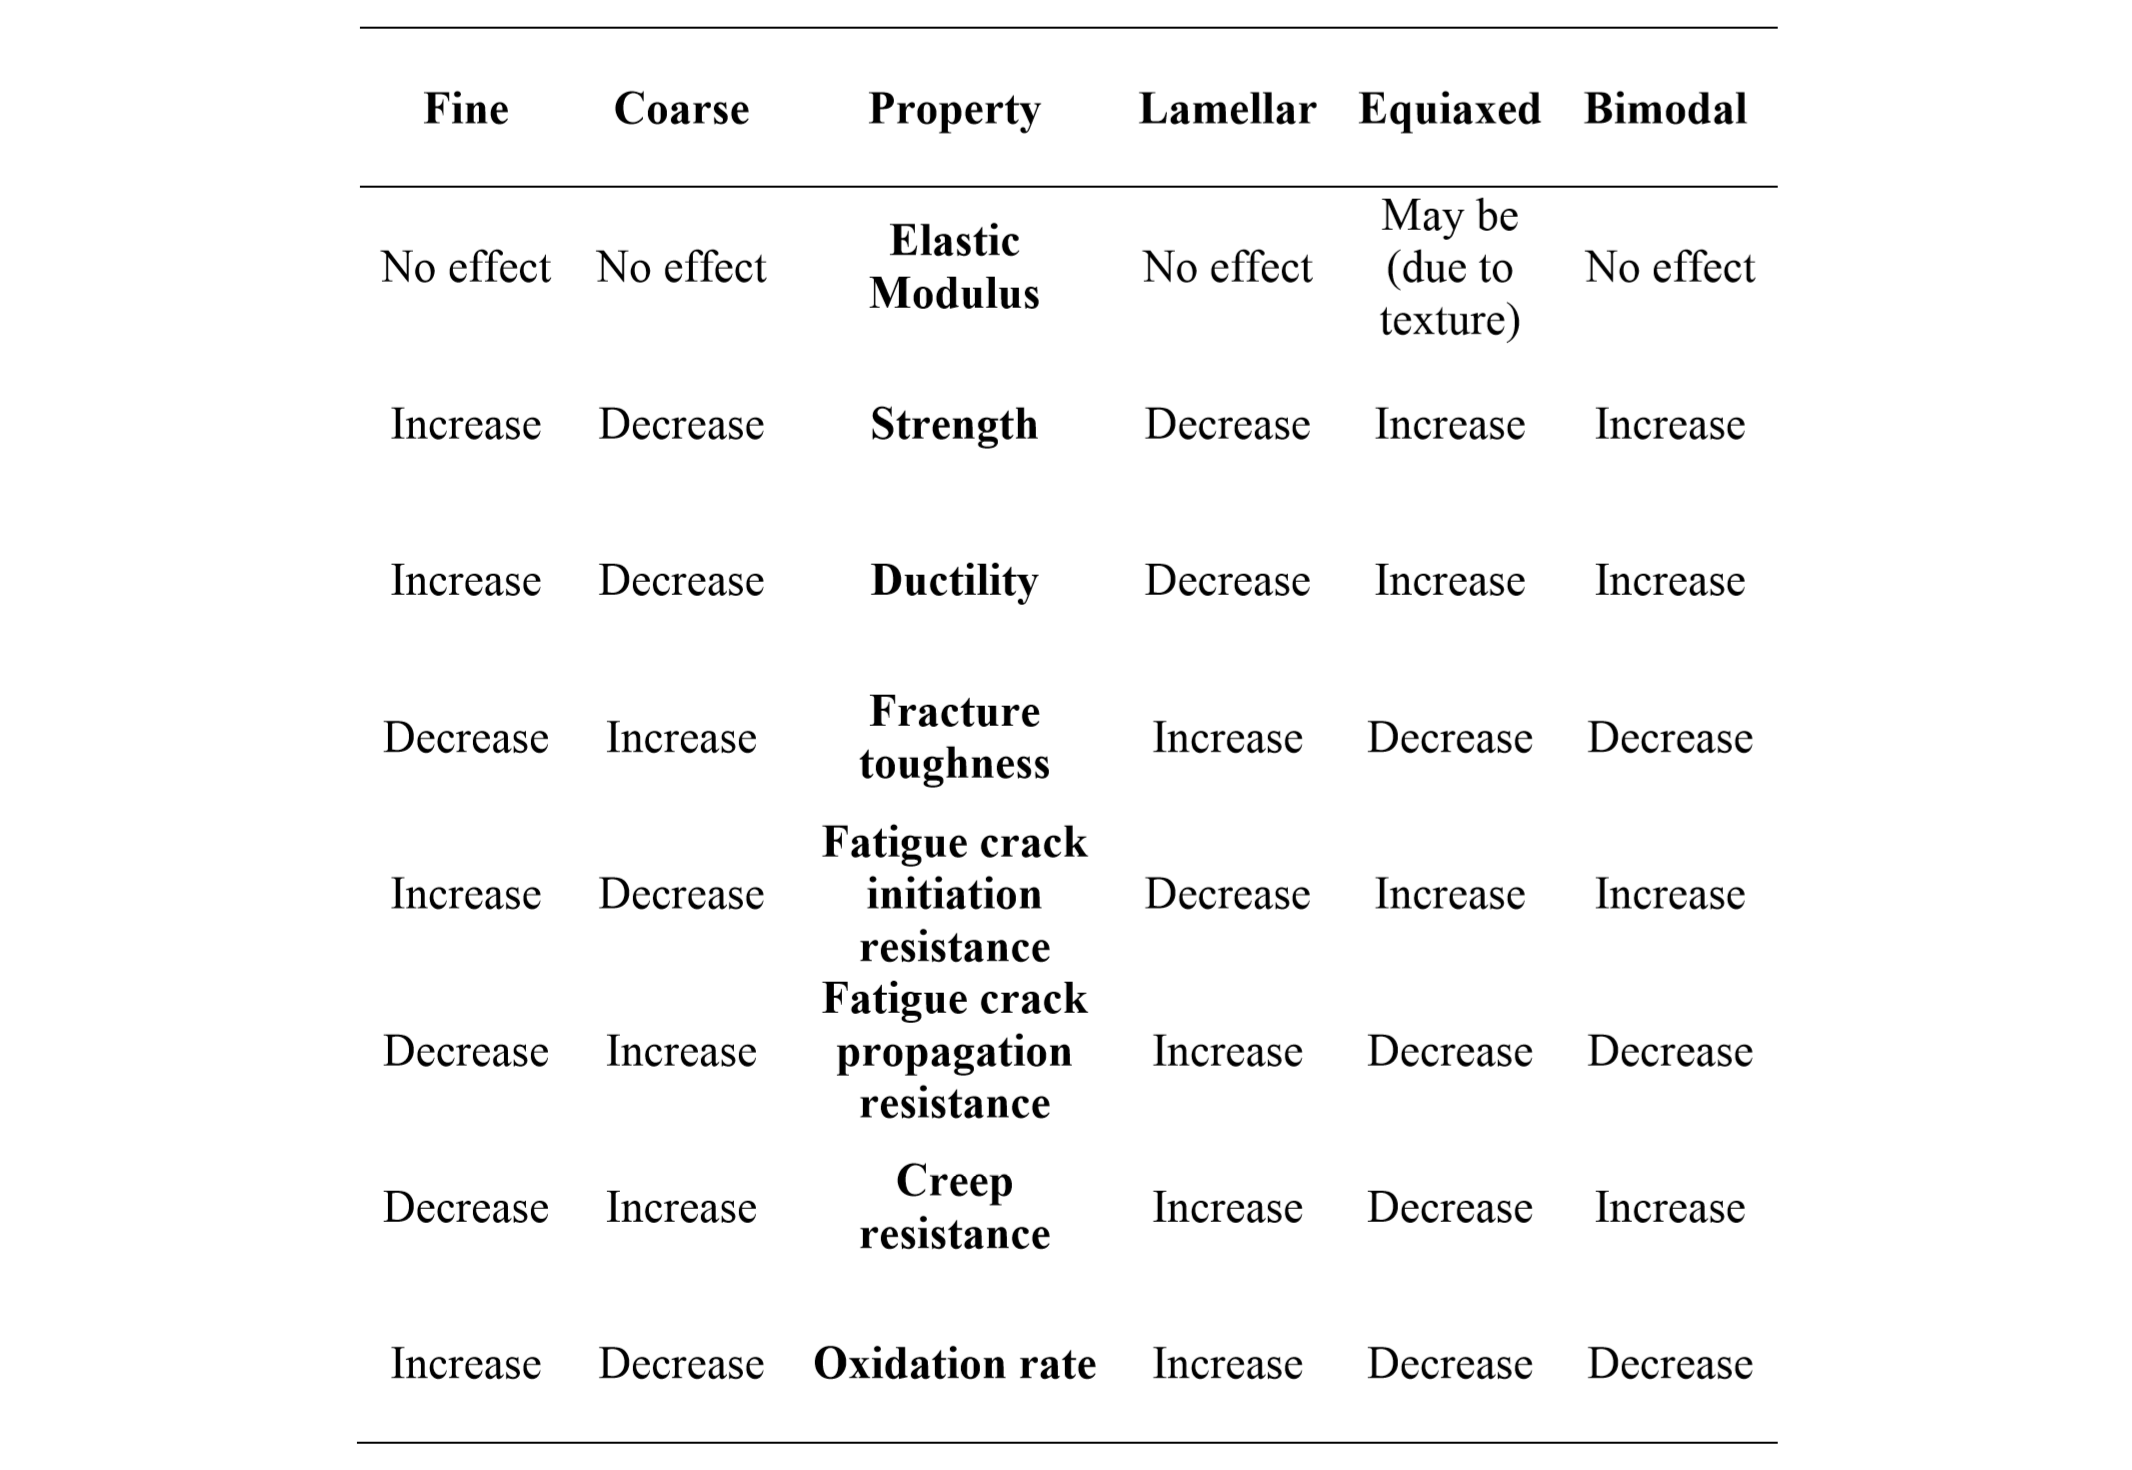
\includegraphics[width=0.9\linewidth]{./Bilder/Tabelle 3.png}
	\caption[Tabelle]{Effekt der Mikrostrukturen auf die mechanischen Eigenschaften in Abhängigkeit der Größe \cite{Boyer.2007}}
	\label{fig:tabelle-3}
\end{figure}

\pagebreak

\subsection{Verwendung von Titan und Titanlegierungen}
Titanlegierungen werden hauptsächlich in der Luftfahrt- und Raumfahrt verwendet, da sie eine gute Kombination aus einem niedrigem Gewicht, hoher Festigkeit, Korrosionsbeständigkeit und einer hohen Temperaturstabilität bieten \cite{C.Leyens.2005,R.R.Boyer.1996,M.PetersJ.KumpfertC.WardC.Leyens.2003}. Die Haupteinsatzgebiete in der Luftfahrt für Titanlegierungen sind Strukturteile der Luftfahrzeugzelle, Fahrwerksteile sowie Komponenten von Flugtriebwerken. Etwa 7 -- 36 \% des strukturellen Gewichts des Rumpfes und der Triebwerke bestehen aus Titanlegierungen \cite{Lutjering.2007}. In Triebwerken werden sie für Triebwerksschaufeln eingesetzt. Für die meisten Komponenten wird die Standardlegierung Ti-6Al-4V verwendet. Für Komponenten, die eine höhere Temperaturbeständigkeit erfordern, werden Legierungen wie Ti–6Al–2Sn–4Zr–2Mo und IMI 834 eingesetzt. Die hohen Material- und Herstellungskosten verhindern einen breiten Einsatz von Titanwerkstoffen in der Automobilindustrie. Sie werden aber vereinzelt für Motorkomponenten oder Fahrwerksteile, wie beispielsweise Federn benutzt. Technisch reines Titan (CP-Titanium) findet Anwendung in Bereichen, wo die Anforderungen an mechanische Eigenschaften gering, aber eine hohe Korrosionsbeständigkeit gefordert ist. Beispiel dafür sind Wärmetauscher, Rohrleitungen oder Meerwasserentsalzungsanlagen \cite{A.D.KhawajiaI.K.KutubkhanahaJ.M.Wieb.2008}. Des Weiteren finden CP-Titanium und Titanlegierungen Anwendung in der Medizintechnik, aufgrund der Biokompatibilität von Titan, sowie einer guten Dauerfestigkeit und Korrosionsbeständigkeit. Sie werden zur Herstellung von Implantaten sowie medizinischen Geräten benutzt \cite{M.GeethaA.K.SinghR.AsokamaniA.K.Gogia.2009}. Ein weiteres Einsatzgebiet sind moderne Schutzwesten, die neben den Aramidfasern auch Titangewebe enthalten, um das Eindringen von Hieb- und Stichwaffen zu verhindern \cite{C.Leyens.2005}.  



\section{Ti-6242 (ZB)}

\subsection{Zusammensetzung}
Ti-6242 ist eine $\alpha$+$\beta$-Titanlegierung, die im Jahr 1967 von TIMET eingeführt wurde \cite{ImmanuelFreiherrvonThungen.}. 
Wie es im Phasendiagramm in \ref{tab:PD-Ti6242} zu erkennen ist, hat die Legierung Ti-6242 bei Raumtemperatur einen hohen $\alpha$-Anteil und wird deshalb als near-$\alpha$-Legierung bezeichnet.
Die genauen Anteile der Legierungselemente kann der Tabelle \ref{tab:Zusammensetzung} entnommen werden. 


\begin{figure}[H]
	\centering
	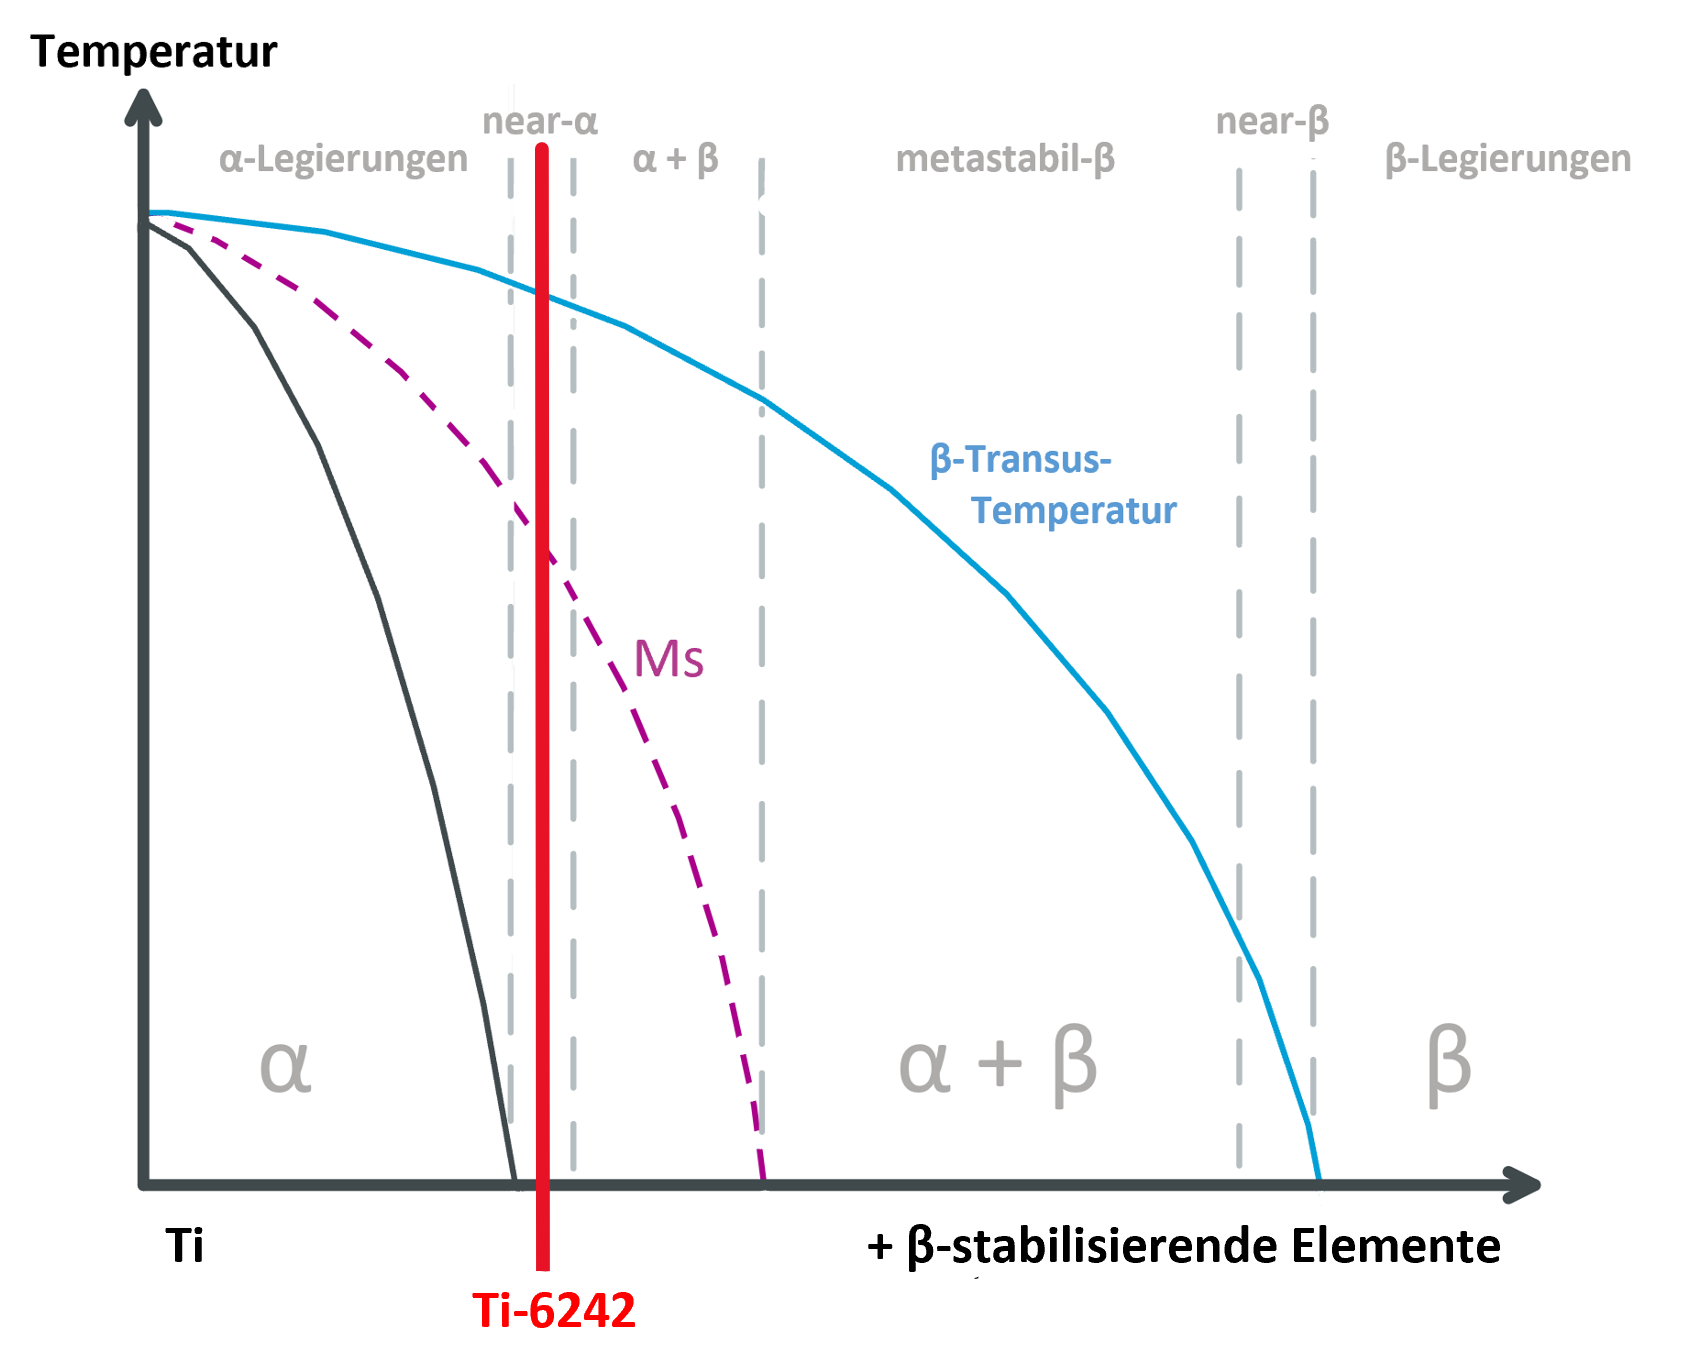
\includegraphics[width=0.5\textwidth]{Bilder/Phasendiagram}
	\caption{Phasendiagramm \cite{M.J.Donachie.2010}}
	\label{tab:PD-Ti6242}
\end{figure}





\begin{table}[H]
	
	\centering	
	\begin{tabular}{|l |c |c|}
		\hline
		\hspace{20ex}Elements \hspace{20ex} & Min \%Gwt. & Max \%Gwt.\\
		\hline
		Aluminium&5,5&6,5\\
		Tin&1.80&2.20\\
		Zirconium&3.60&4.40\\
		Molybdenum&1.80&2.20\\
		Silicon &0.06&0.13\\
		Iron&-&0.25\\
		Oxygen&-&0.15\\
		Carbon&	-&	0.05\\
		Nitrogen&-&0.03\\
		Hydrogen&-&0.0125\\
		
		Titanium &&Remainder\\
		\hline
	\end{tabular}
	\caption{Zusammensetzung von Ti-6242 \cite{M.J.Donachie.2010}}
	\label{tab:Zusammensetzung}
\end{table}
\

Die Ti-6242S ist eine Optimierung von Ti-6242, die in den 1970er Jahren  entwickelt wurde. Zusätzliches Silizium wird in kleinen Mengen zulegiert, um die Resistenz gegen Kriechen vor allem bei hohen Temperaturen durch die Bildung von Siliziden ($Ti_5Si_3$) zu erhöhen. \cite{C.Leyens.2005} 

%Verzeichnis : [Immanuel Freiherr von Thungen] - Immanuel Freiherr von Thungen. Effet dwell: relation microstructure-microtexture-propriétés mécaniquesdel’alliagedetitaneTi6242. Autre. ISAE-ENSMAEcoleNationaleSupérieuredeMécanique et d’Aérotechique - Poitiers, 2016. Français. NNT: 2016ESMA0027 .  tel-01486574

\subsection{Kristallstruktur}

Ti-6242 wird klassischerweise in der bimodalen oder Duplex-Struktur eingesetzt, die nach einer typischen Wärmebehandlung (Abb. \ref{fig:abbildung-7}) erreicht werden kann.

Nach dem Deformationsvorgang wandelt sich bei der Erwärmung von Raumtemperatur  auf eine Temperatur unter $T_{\beta}$  ein Anteil der $\alpha$-Phase in $\beta$ um. Nach einer Haltezeit von $1-2h$ werden die Werkstücke wieder auf Raumtemperatur luftgekühlt.
Dabei wandelt sich das $\beta$ unter Einfluss der Diffusion in $\beta$- und $\alpha$-Lamellen um.

\begin{figure}[H]
	\centering
	\includegraphics[width=0.8\textwidth]{Bilder/Duplexgefüge.jpg}
	\caption{Duplexgefüge bei Ti-6242}
	\label{fig:L.M}
\end{figure}


Als letzte Wärmebehandlung wird klassischerweise  Ti-6242 oder Ti-6242S für  $8 h$ bei $595^\circ C$ angelassen. Dieser Schritt sorgt dafür, dass sich $\alpha_2$ ($Ti_3Al$) in der $\alpha$-Phase ausscheidet und diese dadurch verhärtet. Der Temperaturbereich hängt dabei von der Solvus-Temperatur von $\alpha_2$ in $\alpha$ ab, die ca. $650^\circ C$ beträgt \cite{Lutjering.2007}.
Für besonders gutes Kriechverhalten bei hohen Temperaturen, wird auch die Solvus-Temperatur von Si berücksichtigt, die knapp unter $600^\circ C$ liegt. Silizide ($Ti_5Si_3$) können sich aufgrund ihrer komplexen Kristallstruktur dann in den Korngrenzen ausscheiden und Kornbewegungen verhindern.

\begin{figure}[H]
	\centering
	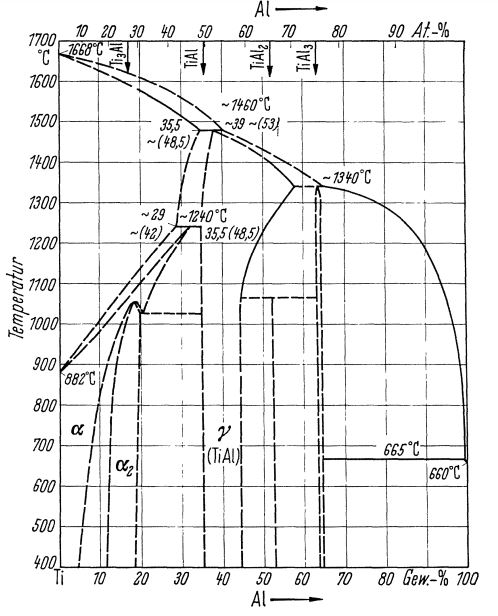
\includegraphics[width=0.6\textwidth]{Bilder/TiAl}
	\caption{Phasendiagramm von Ti-Al . \cite{Zwicker.2014}}
	\label{fig:PD_tial}
\end{figure}

Wärmebehandlungen von Ti-6242 und deren Einflüsse werden in den nächsten Kapiteln genauer diskutiert.


\subsection{Physikalische und mechanische Eigenschaften}

Die Tabelle \ref{Phy.eig.} fasst die physikalischen Kennwerte von Ti-6242 zusammen.


\begin{table}[H]
	\centering	
	\begin{tabular}{l c}
		
		Physikalische Eigenschaften & \\
		\hline
		Dichte& 4,54 g/$cm^3$\\
		Wärmeleitfähigkeit & 7 $W/mK$ \\
		Spezifische Wärmekapazität & 0.460 $J/gK$\\
		Schmelzpunkt & 1700$^\circ$ C \\
		$T_{\beta}$ &  995$^\circ$ C $\pm$ 15$^\circ$ C \\
		
		\hline
		
	\end{tabular}
	\caption{Physikalische Kennwerte von Ti6242 \cite{DavidBenjamin.19801980} \cite{Davis.1990} \cite{Holt.1997}}
	\label{Phy.eig.}
\end{table}

\pagebreak

Die mechanischen Eigenschaften von Titanlegierungen, wie bereits im ersten Kapitel erklärt wurde, hängen auch stark von den verschiedenen Wärmebehandlungen ab, die die Gefügestruktur des Werkstoffes und so auch sein thermomechanisches Verhalten verändern.
Als eine near-$\alpha$-Legierung, besteht Ti-6242 zum größten Teil aus $\alpha$-Phase (90--95\%)(Siehe Phasendiagramm in Abbildung \ref{tab:PD-Ti6242}). Da die Diffusionsrate der $\beta$-Phase höher ist als die der $\alpha$-Phase, weist Ti-6242 eine bessere Stabilität bei höheren Temperaturen auf. \cite{Prasad.2017} 

\begin{table}[H]
	\centering	
	\begin{tabular}{|c| c| c| c| c| c|}										
		\hline
		$T_{\beta}$ & Härte[HV] & E-Modul [GPa]& YS [MPa]&TS[MPa]& El \% \\
		\hline
		995&340&114&990&1010&13\\
		\hline
	\end{tabular}
	\caption{Physikalische Kennwerte von Ti-6242S \cite{C.Leyens.2005}}
	\label{Mec.}
\end{table}
	
	Die $\beta$-Transus-Temperatur ($T_{\beta}$) von Ti-6242 liegt bei 995 $\pm$ 15$^\circ$C. Die Toleranz ist durch die Anteilsschwankungen der verschiedenen Legierungselemente bedingt. Wie bereits im ersten Kapitel beschrieben wurde, stabilisieren  Al, O , N und C die $\alpha$-Phase und erhöhen im Gegensatz zu Mo die $T_{\beta}$.
	Aufgrund des niedrigen Mo-Gehalts von Ti-6242 liegt ihre $\beta$-Transus-Temperatur oberhalb der des reinen Titans, die bei 882 $\pm$ 2$^\circ$C liegt.
	

\begin{figure}[h]
		\centering
		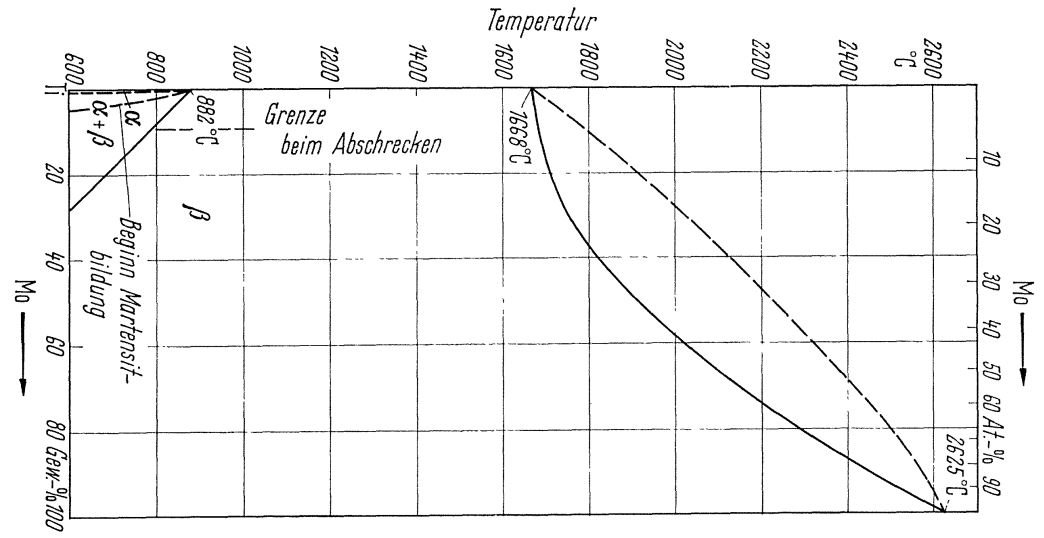
\includegraphics[width= 0.9\textwidth, angle=90]{Bilder/TiMo}
		\caption{Phasendiagramm Ti-Mo \cite{Zwicker.2014}}
		\label{TiMo}
\end{figure}
	
\begin{table}[H]
		\small
		\tabcolsep=0.09cm
		\centering	
		\begin{tabular}{|c |c |c|c |c|}
			\hline
			Thickness[mm] & Tensile strength [MPa] & Yield strengh [MPa] & Elongation[\%]& Reduction in Area [\%]. \\
			\hline
			25-50&1000&930&14&33\\
			102&1000&930&12&30\\
			205&1035&940&12&28\\
			330&1000&825&11&21\\
			
			\hline
	    \end{tabular}
		\caption{Elatische Eigenschaften bei Raumtemperatur von Ti6242Si (Annealed 954$^\circ$C/1h/AC + 600$^\circ$C/8h/AC ) \cite{M.J.Donachie.2010}}
		\label{Mecprop}
\end{table}
	
	
	Alle sekundären Fertigungsverfahren, die für die Herstellung von Bauteilen erforderlich sind, wie z.~B.~ Biegen, Fräsen und Schweißen, können die  Eigenschaften von Titan oder Titanlegierungen stark beeinflussen und müssen daher mitberücksichtigt werden.
	
	
\subsection{Verwendung}
	
	
	Die Kombination der Festigkeit des $\alpha$+$\beta$-Gefüges mit der relativ hohen Kriechbeständigkeit der $\alpha$-Strukturen macht Ti-6242 zu einer Hochtemperaturlegierung. 
	Wegen dieser Eigenschaften wird Ti-6242 hauptsächlich in der Luftfahrt eingesetzt. Vor allem bei rotierenden Teilen im Triebwerk, wo hohe Kriech- und Ermüdungsbeständigkeit neben einer hohen metallurgischen Stabilität bei hohen Temperaturen erforderlich sind. 
	Ti-6242-Bauteile können bei Temeraturen bis zu 550$^\circ C$ eingesetzt werden \cite{C.Leyens.2005}.
	Ti-6242 wird z.B. in der Herstellung von Hochdruckverdichterschaufeln, Turbinenschaufeln und Nachbrennern verwendet, wo neben den oben erwähnten Eigenschaften auch die Korrosionsbeständigkeit bei hohen Temperaturen erforderlich ist. 
	
	
	
	
	
	
	\begin{figure}[H]
		\centering
		\subfloat[Compressor spool for GE CF6 class engine using inertia welding to connect the individual stages: front (smaller) five stages: Ti–6Al–4V; rear two stages: Ti-6242 ]
		{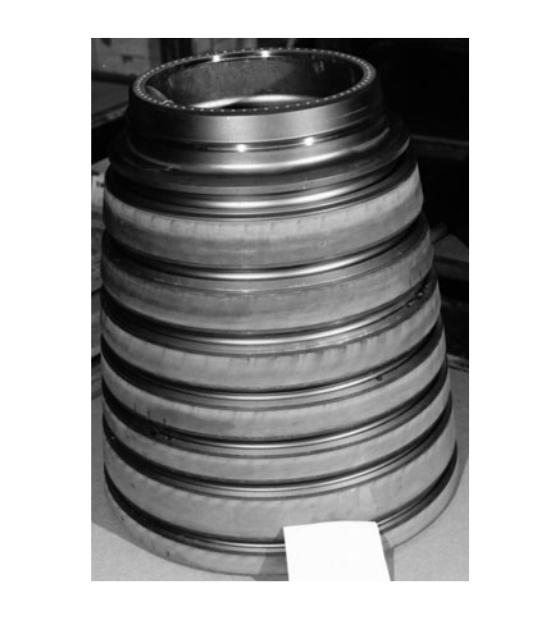
\includegraphics[width=0.45\textwidth]{Bilder/Compressor spool}}
		\hspace{1ex}
		\subfloat[Impeller used in a small engine for regional jets, diameter 35 cm. The alloy is Ti-6242 with a bi-modal microstructure]
		{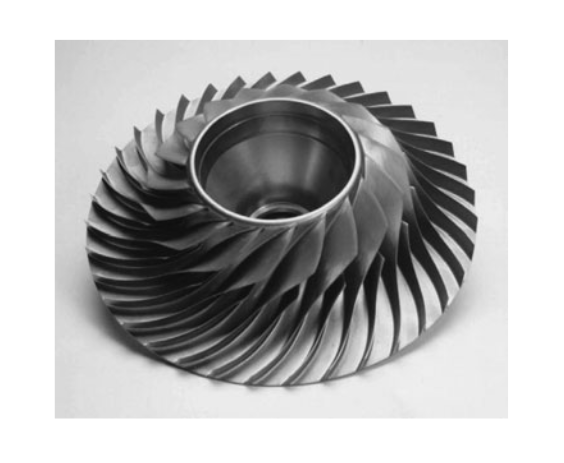
\includegraphics[width=0.45\textwidth]{Bilder/Impeller}}	
		\subfloat[Bläser und Verdichter des JT9D-Triebwerkes, das zu 28 \% des Fluggewichtes aus
		Titan und Titanlegierungen besteht, Bläser aus Ti-Al6-V4, Verdichter mit zunehmender
		Temperatur aus Ti-Al6-V4, Ti-Al6-Sn2-Zr4-Mo2 ]
		{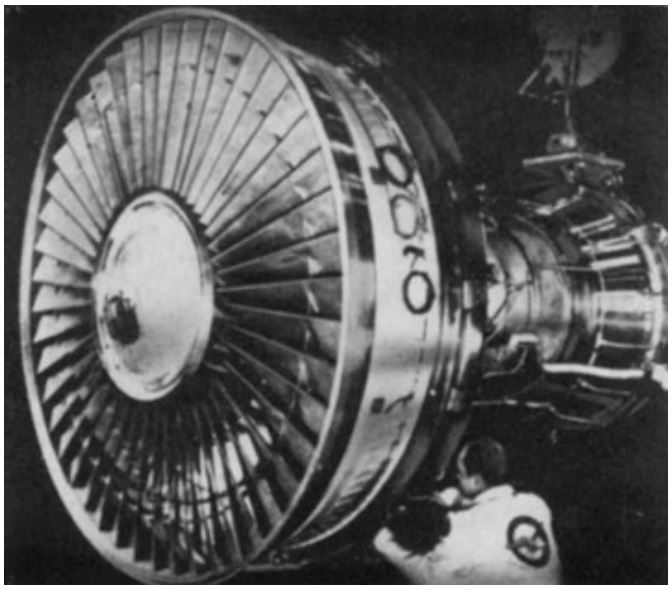
\includegraphics[width=0.45\textwidth]{Bilder/Titan}}
		\caption{Beispiele für Einsatzbereiche von Ti-6242 \cite{Prasad.2017,Zwicker.2014} }
	\end{figure}
